%\documentclass[12pt, draftclsnofoot, onecolumn,letterpaper]{IEEEtran}
\documentclass[12pt, letterpaper]{article}
%\documentclass[12pt, letterpaper]{IEEEtran}
\usepackage{ multirow }
\usepackage{longtable}
\usepackage{geometry}
\usepackage{ragged2e}
\usepackage[table]{xcolor}
\usepackage{booktabs}
\usepackage{graphicx}
\usepackage{caption}
\usepackage{subcaption}
\usepackage{lipsum}
\usepackage{makeidx}
\usepackage{enumerate}
\usepackage{color}
\usepackage{refstyle}
\usepackage{cite}
\usepackage{amsmath}
\usepackage{amssymb}
\usepackage{nomencl}
\usepackage{amsmath}
\usepackage{multirow}
\usepackage{graphicx}
\usepackage{multirow}
\usepackage{anysize}
\usepackage{float}
\usepackage{epstopdf}
\usepackage{threeparttable}
\usepackage{multicol}
\usepackage{amssymb}
\usepackage{adjustbox}
\usepackage{hyperref}
%\usepackage[none]{hyphenat}
%\usepackage{float}

%\usepackage{fixltx2e}
\usepackage{amsmath, amssymb, upgreek, amsthm}
\usepackage{graphicx}
\usepackage{tikz}
\geometry{letterpaper, left=20mm, right=20mm, top=20mm, bottom=20mm}
\usetikzlibrary{patterns} % LATEX and plain TEX when using Tik Z
\allowdisplaybreaks
\setlength{\textfloatsep}{2ex}
\usepackage{array}
\usepackage{enumitem}
\setlength{\parindent}{1 em}
\setlength{\parskip}{0.5 em}
\renewcommand{\baselinestretch}{1.25}
\def\dsd{d_\text{SD}}
\def\Rcoop{R_\text{Coop}}
\def\rhd{R_\text{HD}}
\def\rsd{R_\text{SD}}
\def\rsh{R_\text{SH}}
\def\Pcoops{\mathcal{P}^\text{Succ}_\text{Coop}}
\def\dsh{d_\text{SH}}
\def\dhd{d_\text{HD}}
\def\psibar{\overline{\mathcal{P}}^\text{Succ}_{i}}
\def\psbara{\overline{\mathcal{P}}^\text{Succ}_{1}}
\def\psbarb{\overline{\mathcal{P}}^\text{Succ}_{2}}
\def\psbarc{\overline{\mathcal{P}}^\text{Succ}_{3}}
\def\psbard{\overline{\mathcal{P}}^\text{Succ}_{4}}
\def\psbare{\overline{\mathcal{P}}^\text{Succ}_{5}}
\def\Ri{R_{i}}
\def\Ps{\mathcal{P}^\text{Succ}_\text{Direct}}
\def\frk{\mathrm{f}_{r_k}(r)}
\def\Rcoopj{R_\text{coop}^j}
\title{\bf \vspace*{-4ex} Statement of Responses to the Editor and the Reviewers of Paper-TNSM \\[-6ex]}
\date{}

\begin{document}
%\vspace*{-10ex}
%\sloppy
\maketitle
We would like to thank the editor and reviewers for their comments on our manuscript.
We hope that the modifications that we have made to the manuscript, and the responses that we have
provided herein will alleviate the reviewers' concerns. Below, please find our detailed responses to the editor and reviewers' comments and suggestions.
\\ [-3.ex]
% % % % % % % % % % % % % % % Editor % % % % % % % % % % % % % % % % % % % %


\clearpage
\noindent
\begin{longtable}{|p{0.975\textwidth}|}
\hline \hline
\Centering
\cellcolor{gray!60}
\textbf{Editor} \\
\hline \hline %\hline \hline \hline
\RaggedRight
\cellcolor{violet!15}
\textbf{\noindent  Comments to the Author} ``The paper has gone through three independent reviews and also checked by myself. The topic is interesting and there are merits. But there are some major concerns on the contribution, the assumption, the model derivation, and the experimental results. I hope the review comments are useful for further improving the quality of the paper. I'd therefore recommend the Resubmission''\\
\hline
\end{longtable}

\vspace*{-1\baselineskip}
\noindent \textbf{Response:\\}
We would like to thank the editor for his comment on our manuscript and giving us the opportunity to resubmit it. By utilizing the comments, we enhanced our paper and eliminated problems.

%\begin{longtable}{|p{0.975\textwidth}|}
%\hline \hline
%\RaggedRight
%\cellcolor{green!10}
%[1] F. Patolsky, B. P. Timko, G. Yu, Y. Fang, A. B. Greytak, G. Zheng, and C. M. Lieber, ``Detection, stimulation, and inhibition of neuronal signals with high-density nanowire transistor arrays,'' Science, vol. 313, no. 5790, pp. 1100-1104, 2006.
%\\
%\hline
%\end{longtable}




% % % % % % % % % % % % % % % Reviewer 1 % % % % % % % % % % % % % % % % % % % %
\clearpage
\noindent
\begin{longtable}{|p{.975\textwidth}|}
\hline \hline %\hline \hline \hline
\Centering
\cellcolor{gray!60}
\textbf{Reviewer 1} \\
\hline \hline %\hline \hline \hline
\RaggedRight
\cellcolor{violet!15}
\textbf{\noindent Comments to the Author} ``
The paper proposes resolving the problem of resource allocation to network slices by using a new algorithm applied to the reformulation of the problem. The results seem promising but the paper has some issues. ''\\
\hline
\end{longtable}
\vspace*{-1\baselineskip}
\noindent \textbf{Response:\\}
We would like to thank the reviewer for this manuscript's careful and thorough reading. We hope that the responses provided will ease the reviewer's concerns.

\begin{longtable}{|p{0.975\textwidth}|}
\hline \hline
\RaggedRight
\cellcolor{gray!15}
\textbf{\noindent Comment1:} ``First, the structure of the paper makes it somewhat hard to follow and there are some mistakes in the text. A proofread is required before it can be accepted for publication.   ''\\
\hline
\end{longtable}
\vspace*{-1\baselineskip}
\noindent \textbf{Response:\\}
According to this comment, we have modified the introduction and checked the entire text and correct mistakes. We have shortened the state of the arts and introduced our goal briefly before the main contribution section. We removed additional information and talked more about our work. Also, we add some figures to describe incomprehensible parts. In addition, we provide further explanations.   





\begin{longtable}{|p{0.975\textwidth}|}
\hline \hline
\RaggedRight
\cellcolor{gray!15}
\textbf{\noindent Comment 2:} ``Although the paper demonstrates its claims, the relaxation of conditions from the original problem formulation is not well justified. It is not clear why the initial formulation of the problem is not feasible and the reformulated makes it feasible while retaining some level of quality of the solutions given. A deeper analysis of both formulations must be presented. ''\\
\hline
\end{longtable}
\vspace*{-1\baselineskip}
\noindent \textbf{Response:\\}
I would appreciate your comments to enhance and clarify this section of the paper.

The problem (13) is feasible and has feasibility points discussed in Subsection IV-B, and we introduce a fast algorithm (i.e., Algorithm 3 in Subsection IV-B) for feasibility points. Although the problem is feasible, it is not convex and challenging to solve. Since problem (13) is mixed-integer nonlinear programming with two integer variables, the PRB assignment, $e$, and the number of VNFs in slice $s$, $M_s$, and by relaxing the variables, the problem is also non-convex; therefore, this problem is NP-hard. Solving the problem is not trivial. To solve the problem by inspiring Stackelberg, we reformulate the equation in (13g) to reduce one of the variables (i.e., $M_s$) that can be solved after obtaining the rate of UEs. We notice that $M_s$ is similar to the followers in Stackelberg Competition, and power and PRB assignment are identical to the leader. So, the new problem has two variables: power and PRB assignment. This new problem is convex by relaxing the binary variable, the PRB assignment, and estimating the lower bounds (15). The objective function and constraints of the problem are convex and can be solved by the Lagrangian function. After obtaining the power of UEs and PRB assignment, we can obtain the achievable rate of each UE so we can find the optimal number of VNFs in each slice ($M_s$). We made changes in Subsection III-A, accordingly.


\begin{longtable}{|p{0.975\textwidth}|}
\hline \hline
\RaggedRight
\cellcolor{gray!15}
\textbf{\noindent Comment3:} ``Moreover, the baseline and FBDR methods used in the comparison are not well introduced. They are vaguely linked to related work but not as needed. The paper must clarify the relation of the related work and the compared alternatives. The paper must also contextualize the proposal among the related work by comparing their qualities and/or performance.  ''\\
\hline
\end{longtable}
\vspace*{-1\baselineskip}
\noindent \textbf{Response:\\}
We would like to thank the reviewer for emphasizing this point and helping us with a better exhibition. 

 Two different methods are used to compare with the performance of the proposed method (IABV) and show the optimality of our approach.

 The first one is a baseline scheme, which uses random PRB allocation. Therefore, the allocation of PRB to each UE is random when we have low interference, but in figures with high interference, we randomly assign just one RB to each UE. Also, the association of O-RU is carried out based on distance. It means that each UE is assigned to the nearest O-RU. The optimal power is obtained using the CVX of Matlab, which uses the successive convex approximation (SCA) method since the problem is convex.
After achieving power and other parameters, the achievable rate will be obtained, and the optimal number of VNF is achieved from Lemma (1). 

For the second one, we use the idea of the fixed BBU capacity and dynamic resource allocation (FBDR) algorithm proposed in [18] and named it the dynamic resource allocation scheme (DR scheme). 
 We have services with different QoS in this work, similar to tenants with different QoS introduced in [18]. Therefore, we can use the DR scheme similar to the FBDR method adapted to our conditions for comparison. Instead of BBU in C-RAN, we have O-DU and O-CU in O-RAN.
 Since we do not talk about O-DU and O-CU capacity, we use the dynamic resource allocation scheme (DR scheme) algorithm and do not consider BBU capacity.
But also, we can assume that O-DU and O-CU have fixed sufficient capacity in our system model. Also, our mid-haul link (F1 link) has adequate capacity, so there will be no issue using the idea of the FBDR method with this assumption and using the DR scheme. In the DR scheme, PRB and power are dynamically allocated. The number of VNFs is obtained from the simulation. The UEs are associated with the O-RU based on the quality of their channels and the channel distance instead of using the greedy algorithm 1 (GAA algorithm) for O-RU assignment. The figures in [18] show that dynamic BBU capacity and dynamic resource allocation (DBDR) perform better than FBDR for the same priority area. The numerical results section also indicates that our proposed algorithm performs better than the DR scheme.

We add this response in subsection IV-A.


\begin{longtable}{|p{0.975\textwidth}|}
\hline \hline
\RaggedRight
\cellcolor{gray!15}
\textbf{\noindent Comment4:} ``Finally, the source of the values used for the parameters in the evaluation must be clarified.  ''\\
\hline
\end{longtable}
\vspace*{-1\baselineskip}
\noindent \textbf{Response:\\}

We refer to the following list of references in our numerical result for this comment:

\begin{longtable}{|p{0.975\textwidth}|}
\hline \hline
\RaggedRight
\cellcolor{green!10}
[1] 3GPP-TS-36.104-V13.3.0, “Evolved Universal Terrestrial Radio Access (E-UTRA);
Base Station (BS) radio transmission and reception
(Release 13),” 2016-03.

[2]  3GPP-TR-36.931-V13.0.0, “Technical Specification Group Radio Access Network;
Evolved Universal Terrestrial Radio Access (E-UTRA);
Radio Frequency (RF) requirements for LTE Pico Node B
(Release 13),” 2016-01.

[3] 3GPP-TS-25.101-V4.13.0, “User equipment (UE) radio transmission
and reception (FDD)(release 4),” 2006-12.

[4]E. Mohyeldin, “Minimum technical performance requirements for
imt-2020 radio interface(s),” 2020.

[5]  ETSI-TR-138-913-V14.3.0, “5G; study on scenarios and require-
ments for next generation access technologies(3GPP TR 38.913 version
14.3.0 release 14),” 2017-10.

\\
\hline
\end{longtable}

In [1 page 11], the amount of BW is explained. In [2], the noise power is represented. The amount of delay for eMBB and URLLC are listed on Pages 24 and 25 in [5]. Also, on Page 26, the mMTC packet size is stated. On Page 25, the URLLC packet size is stated.
In [3], on Page 13, Table 6.1, the maximum power is stated. In [4], on Page 4, the delay of URLLC and eMBB is and also the spectral efficiency of eMBB is noted.

We add these references in IV-A (references [41]-[45]).
%%%%%%%%%%%%%%%%%%%%%%%%%%%%%%%%%%%%%%%%%%%%%%%%%%%%%%%%

\clearpage
\noindent
\begin{longtable}{|p{0.975\textwidth}|}
\hline \hline
\Centering
\cellcolor{gray!45}
\textbf{Reviewer 2} \\
\hline \hline
\RaggedRight
\cellcolor{violet!15}
\textbf{\noindent Comments to the Author:} ``The paper focus on the aspect of network slicing in 5G cellular network which entails a service aware resource allocation of the different required virtual network functions (VNFs) for different slices which have different characteristics. More specifically, the paper proposes a mixed integer mathematical problem which in the original form is non-linear and hence hard to solve. To tackle this challenge the optimization problem is decomposed into two sub-problems where the solutions are not optimal however numerical investigations show that the solutions are competitive. In general, the paper is well written and structured.''\\
\hline
\end{longtable}
\vspace*{-1\baselineskip}
\noindent \textbf{Response:\\}
It is our pleasure to thank the reviewer for the careful reading of this manuscript, providing thoughtful comments, and offering constructive suggestions that strengthened and enhanced its quality. We hope that the responses provided herein can alleviate the reviewer's concerns.




\begin{longtable}{|p{0.975\textwidth}|}
\hline \hline
\RaggedRight
\cellcolor{gray!15}
\textbf{\noindent Comment 1:} ``In terms of taking the actual delay in the proposed there are some concerns which might be important for some time critical applications especially in the ultra-reliable low latency communications (URLLC) but also for different applications that fall under the enhanced mobile broadband (eMBB) generic service framework. First of all, in the paper the authors only consider processing delay and ignore propagation and transmission delay. Since multiple paths in reality could be utilized the role of the above two components might play an important role. Nevertheless, the authors need to clearly mention why those two components are not considered, saying for example are constant is not a good enough reason to be ignored since as eluded those change based on routing decisions.''\\
\hline
\end{longtable}
\vspace*{-1\baselineskip}
\noindent \textbf{Response:\\}
We would like to thank the reviewer for this comment to add more detail to our paper regarding end-to-end delays.

Taking propagation and transmission delays into formulations is straightforward, but we avoided that for the sake of better presentation. However, they can be added to the system model easily. In this paper, we focus only on the processing delay to find the optimal number of VNFs, and we consider the other two delays are fixed. We discuss these two types of delay in detail below and explain why we do not consider them in our work.

The propagation delay is considered when each O-RU can connect to the number of O-DUs and can select to connect to which O-DU based on the route, capacity, and priority. Also, the connections of O-DUs to O-CUs are the same as O-RU to O-DU. Therefore, different routes will be added to the system to solve the routing problem. Also, for URLLC and mMTC, edge processing can reduce the delay that is not considered here.
However, it provides a new problem formulation and can be added to our system model to extend our paper in the future. Thus, this paper assumes that the connection between O-RUs and O-DUs is fixed and transparent, and we do not consider the problem of edge processing. As a result, the propagation delay is fixed and does not affect the optimization problem. The following is a brief calculation of propagation and transmission delay.
Since the distance between the O-RU and O-DU is about 10 km and also the distance between O-DU and O-CU is about 80 km. Moreover, the distance from O-CU to the network should not exceed 200 Km [35]. so, the propagation delay is about $T^{\text{pro}} = (10 + 80 + 200)\times 10^3 /(3\times 10^8) < 1ms $. Since fronhaul, midhaul, and backhaul are fiber optics, c is the speed of light. Also, due to the edge technique in O-DU or O-CU for users with low latency, this amount of latency is greatly reduced. But we also do not focus on edge processing in this paper. You can find more about these distances in this \href{https://blogs.keysight.com/blogs/inds.entry.html/2020/06/30/5g_testing_what_is-0nzj.html\%23:~:text=The\%20data\%20requirements\%20are\%20about,DUs\%20is\%20about\%2080\%20km.}{link}.

The following is a brief calculation of transmission delay to show that it does not affect the optimization since it has a small amount.
In URLLC and mMTC, the mean packet size can be between 20 to 32 byte; Also, the minimum data rate is assume to be $46 \frac{bit}{\frac{sec}{Hz}} \times BW (180 KHz)$. So the transmission delay from O-RU to O-DU is about $T^{fr,t} = \frac{20\times 8}{46 \times 180 \times 10^3} < 2 us$. As a result, the $T^{fr,t} \approx T^{mid,t} \approx T^{b,t}$. for eMBB, the packet size can be 100 times larger and the delay is not exceed the 0.6ms.  

We add this response in subsection II-D.



\begin{longtable}{|p{0.975\textwidth}|}
\hline \hline
\RaggedRight
\cellcolor{gray!15}
\textbf{\noindent Comment 2:} ``Also, note that for calculating processing delay requests for different services arriving at blade servers for vnf applications might get different treatment on how they access VMs or containers hence a single queue with non-priority and/or preemption (m/m/1) might not be a good approximation on the performance.''\\
\hline
\end{longtable}
\vspace*{-1\baselineskip}
\noindent \textbf{Response:\\}
The processing delay can be modeled as an M/M/1 queue; since the system's arrival packets are from many independent sources. Moreover, the impact of a single packet on the system's performance is minimal. Also, the queue discipline will be first-in, first-out (FIFO), and the arrival packet is assumed to follow a Poisson process. The system's clock is constant, and the size of the tasks is not fixed. So, we suppose that service times are exponentially distributed [36]. In addition, we assume that the arrival packets of each service have the same priority (in subsection II-F, we will talk about priority), and we consider priority between services, not between UEs of one service. As we assume that the UEs of a service have the same priority, their sent packets also have an equal priority. In addition, since the services are isolated, the UEs in each service have the same priority, and the processing delays of each service are independent of the other services; if we assume service priority, this priority does not invalidate the queueing theory. Therefore, one service could have a higher priority, affecting the whole optimization, and the M/M/1 queue theory is still validated.

We add this response in subsection II-D-1.


\begin{longtable}{|p{0.975\textwidth}|}
\hline \hline
\RaggedRight
\cellcolor{gray!15}
\textbf{\noindent Comment 3:} ``Also worth noting, that later on in the problem formulation there is the notion of service priority $\delta_s$ for data rate but this seems not to be used for accessing cloud resources. For example one could have changed the optimization problem and considered average allocated transmission rate and optimize with the same priorities access to cloud resources (instead of allocating equal access to vnf resources).''\\
\hline
\end{longtable}
\vspace*{-1\baselineskip}
\noindent \textbf{Response:\\}
We would like to thank the reviewer for the great suggestion they gave us.
Since the priority is in the objective function of the equation (13), the priority has affected the whole optimization problem.
Therefore, priority is given to the whole optimization problem, and the optimization problem obtains the number of VNFs by affecting the priority term. If we were to discuss the placement of VNFs on the data centers, the problem would become a knapsack or bin-packing problem, and here the prioritization would affect the resource allocation algorithm, including memory, RAM, CPU, and bandwidth of VNFs. Therefore, the algorithm was implemented based on prioritization. But, in this paper, we consider priority more generally. This is an excellent suggestion for extending this paper in the future. Hence, in the extension of the paper, we would talk about VNF placement, and the priority will be more different from here, and the access of VNF resources will be based on the priority.


\begin{longtable}{|p{0.975\textwidth}|}
\hline \hline
\RaggedRight
\cellcolor{gray!15}
\textbf{\noindent Comment 4:} ``Some form of rationalization should be given for abstracting Interference as Gaussian noise. This is important because we expect the system to be interference limited and cell edge users to experience significant different levels of performance compared to centre cell users.''\\
\hline
\end{longtable}
\vspace*{-1\baselineskip}
\noindent \textbf{Response:\\}
 $I_{r,u(s,i)}^{k}$ is the sum of the power of interfering signals and quantization noise represented as follow
%{\color{red} use paranthesis in the following equation to clear +}
\begin{subequations}\label{eqI}
\begin{alignat}{4}
&I_{r,u(s,i)}^{k} =\\
 &\underbrace{\sum_{\substack{l=1 \\ l\neq i}}^{{U}_{s}} e^{k}_{u(s,i)}e^{k}_{u(s,l)}  p_{u(s,l)}^{k}\sum_{\substack{r'=1 \\ r'\neq r}}^{R}|{\bold{h}_{r',u(s,i)}^{H \: k}} \bold{w}_{r',u(s,l)}^{k} g_{u(s,l)}^{r'}|^2}_{\text{(intra-slice interference)}}+\\
&\underbrace{\sum_{\substack{n = 1 \\ n\neq s}}^{S}\sum_{l=1}^{{U}_s} e^{k}_{u(s,i)}e^{k}_{u(n,l)}  p_{u(n,l)}^{k}\sum_{\substack{r'=1 \\ r'\neq r}}^{R}|{\bold{h}_{r',u(s,i)}^{H \: k}} \bold{w}_{r',u(n,l)}^{k} g_{u(n,l)}^{r'}|^2}_{\text{(inter-slice interference)}}\\
&+\underbrace{  \sum_{j=1}^{{R}} {\sigma_q}^2 |\boldsymbol{h}_{r,{u(s,i)}}^k|^2 }_{\text{(quantization noise)}},
\end{alignat}
\end{subequations}
%{\color{red} $\gamma_1$ is constant used instead of variable. }
%where $\gamma_{1} = e^{k}_{u(s,i)}e^{k}_{u(s,l)}$ and $\gamma_{2} = e^{k}_{u(s,i)}e^{k}_{u(n,l)}$.
where $e^{k}_{u(s,i)}$ is the binary variable to show whether the $k^{th}$ PRB is allocated to the UE $i$ in slice $s$, assigned to $r^{th}$ O-RU. %($\gamma_1$ and $\gamma_2$ are two variales. You  define on variable here.)
Furthermore, there is no inter-slice interference since slices are isolated and there is just intra-slice interference.

Here we have two Gaussian noise types: additive Gaussian noise and the other is Gaussian quantization noise. The second noise is added to the interfering signal and shown with $ I_{r,u(s,i)}^{k}$ and it is different with interference.
To obtain SNR as formulated in equation (1) in the paper, let $y_{u(s,i)} $ be the received signal of UE $i$ in $s^{th}$ service formulated as
\begin{equation}\label{eq2}
y_{u(s,i)} = \sum_{r = 1}^{R}\sum_{k=1}^{K_s} \boldsymbol{h}^{H \: k}_{r,u(s,i)} g_{u(s,i)}^r e^k_{r,u(s,i)}{x_Q}^k_{r,u(s,i)}+ z_{u(s,i)},
\end{equation}

%\boldsymbol{w}^k_{r,u(s,i)}p^k_{r,u(s,i)}  $\mathfrak{y}^k_{r,u(s,i)} =\boldsymbol{w}^k_{r,u(s,i)}{p^{k \: \frac{1}{2}}_{r,u(s,i)}} x_{u(s,i)}+ \boldsymbol{q}_{r}$
where ${x_Q}^k_{r,u(s,i)} ={x_P}^k_{r,u(s,i)}+ \boldsymbol{q}_{r}$. Also, ${x_P}^k_{r,u(s,i)}= \boldsymbol{w}^k_{r,u(s,i)}{p^{k \: \frac{1}{2}}_{r,u(s,i)}} x_{u(s,i)} $, and  $ x_{u(s,i)}$ depicts the transmitted symbol vector of UE $i$ in $s^{th}$ set of service,  $z_{u(s,i)}$ is the additive Gaussian noise $z_{u(s,i)} \backsim \mathcal{N}(0,N_0)$ and $N_0$ is the noise power.
Moreover, ${x_P}$ denotes the precoded message before compression, and ${x_Q}$ illustrates the precoded message after compression that is shown in figure \ref{fig:pq}. 
In addition, $\boldsymbol{q}_{r} \in \mathbb{C}^{J }  $ indicates the quantization Gaussian noise 
($\boldsymbol{q}_{r} \backsim \mathcal{N}(0,{\sigma_q}^2\boldsymbol{I_{R}} )$), which is made from signal compression in O-DU.
\begin{figure}
  \centering 
  \captionsetup{justification=centering}
    \includegraphics[scale = 0.7]{Qdiag.png}
    %\includegraphics[max height=30cm,max width=9.5cm]{Drawing15.eps}
    %\includegraphics[width=\textwidth]{finalDraw.pdf}
  \caption{Precoding and Quantization of Signal}
  \label{fig:pq}
\end{figure}

We add this response in subsection II-B.


\begin{longtable}{|p{0.975\textwidth}|}
\hline \hline
\RaggedRight
\cellcolor{gray!15}
\textbf{\noindent Comment 5:} ``Constraint 13n (changed to 13k in new version) is not clear - it means that there are VMs and/or containers available in the network and an operator denies service due to an energy consumption budget (which again is not very detailed to capture the actual energy consumption of each node/vnfs under different loads etc.). In general the subsection on VNF power consumption is very limited in scope. ''\\
\hline
\end{longtable}
\vspace*{-1\baselineskip}
\noindent \textbf{Response:\\}
{We thank the reviewer for adding clarity to our paper and reducing ambiguity in this condition in response to this comment.
A significant issue facing the industry is reducing energy consumption. Data centers are one of the most energy-consuming. As a result, restrictions are placed on data centers' energy, including virtual machines (VMs). So, one of our goals is to limit the energy consumption of total VNFs that can be run as VM on data centers. Therefore, by applying a custom policy on total power consumption, we can control data centers' power consumption ($\phi^{\text{\text{tot}}}  \leq \phi^\text{max}$).

We add this response in subsection II-E.

\clearpage
\noindent
\begin{longtable}{|p{0.975\textwidth}|}
\hline \hline
\RaggedRight
\cellcolor{gray!15}
\textbf{\noindent Comment 6:} ``Some rationalization is needed on why the packet size is considered to be 20 bytes. ''\\
\hline
\end{longtable}
\vspace*{-1\baselineskip}
\noindent \textbf{Response:\\}
Thank for this important comment. Our simulation parameters were based on [42-46], and in particular, for this parameter, we used the following reference 
We refer to the following reference in our numerical result for this comment:

\begin{longtable}{|p{0.975\textwidth}|}
\hline \hline
\RaggedRight
\cellcolor{green!10}
[1]  ETSI-TR-138-913-V14.3.0, “5G; study on scenarios and require-
ments for next generation access technologies(3GPP TR 38.913 version
14.3.0 release 14),” 2017-10.

\\
\hline
\end{longtable}

On [1, Page 25], the URLLC packet size is stated to be 32 bytes, and on Page 26, the packet size of mMTC is stated to be 20 bytes. We changed the URLLC packet size to 32, but it has little impact on the simulation result.

We add this reference in IV-A (reference [45]).

\begin{longtable}{|p{0.975\textwidth}|}
\hline \hline
\RaggedRight
\cellcolor{gray!15}
\textbf{\noindent Comment 7:} ``Comparison with [18] might not be fair since that work also considers BBU capacity and also performs admission control functionalities, also there are different tenants that have different users with variable required QoS. ''\\
\hline
\end{longtable}
\vspace*{-1\baselineskip}
\noindent \textbf{Response:\\}
We appreciate the reviewer emphasizing this point and providing us with tips on how to improve our paper.
 
For the second one, we use the idea of the fixed BBU capacity and dynamic resource allocation (FBDR) algorithm proposed in [18] and named it the dynamic resource allocation scheme (DR scheme). 
 We have services with different QoS in this work, similar to tenants with different QoS introduced in [18]. Therefore, we can use the DR scheme similar to the FBDR method adapted to our conditions for comparison. Instead of BBU in C-RAN, we have O-DU and O-CU in O-RAN.
 Since we do not talk about O-DU and O-CU capacity, we use the dynamic resource allocation scheme (DR scheme) algorithm and do not consider BBU capacity.
But also, we can assume that O-DU and O-CU have fixed sufficient capacity in our system model. Also, our mid-haul link (F1 link) has adequate capacity, so there will be no issue using the idea of the FBDR method with this assumption and using the DR scheme. In the DR scheme, PRB and power are dynamically allocated. The number of VNFs is obtained from the simulation. The UEs are associated with the O-RU based on the quality of their channels and the channel distance instead of using the greedy algorithm 1 (GAA algorithm) for O-RU assignment. The figures in [18] show that dynamic BBU capacity and dynamic resource allocation (DBDR) perform better than FBDR for the same priority area. The numerical results section also indicates that our proposed algorithm performs better than the DR scheme.

We add this response in subsection IV-A.


\begin{longtable}{|p{0.975\textwidth}|}
\hline \hline
\RaggedRight
\cellcolor{gray!15}
\textbf{\noindent Comment 8:} ``Also, interference is measured in a more detailed manner (maximum interference per UE) and hence when this relaxed (Guassian noise) the performance expected to slightly increase. Hence, some more detailed discussion on what has been assumed is needed. ''\\
\hline
\end{longtable}
\vspace*{-1\baselineskip}
\noindent \textbf{Response:\\}
Here we have two Gaussian noise types: additive Gaussian noise and the other is Gaussian quantization noise which is shown in Fig \ref{fig:pq}. We offer the sum of interference and the Gaussian quantization noise with $ I_{r,u(s,i)}^{k}$. Also, the Gaussian quantization noise is independent of interference and related to channel gain of UEs.

We add this response in subsection II-B.
%%%%%%%%%%%%%%%%%%%%%%%%%%%%%%%%%%%%%%%%%%%%%%%%%%%%%%%%%

\clearpage
\noindent
\begin{longtable}{|p{0.975\textwidth}|}
\hline \hline
\Centering
\cellcolor{gray!45}
\textbf{Reviewer 3} \\
\hline \hline
\RaggedRight
\cellcolor{violet!15}
\textbf{\noindent Comments to the Author} ``The authors propose a resource allocation scheme for network slicing in an Open RAN scenario. They consider three network slice types namely eMBB, URLLC and mMTC and provide a solution for end-to-end slicing considering resource allocation over the RAN domain following the proposed ORAN architecture, as well as VNF allocation. In general, the paper is well written, however some parts need to be rephrased and restructured.''\\
\hline
\end{longtable}
\vspace*{-1\baselineskip}
\noindent \textbf{Response:\\}
We would like to thank the reviewer for careful and thorough reading of our manuscript and for
the thoughtful comments and constructive suggestions, which helped us to improve
the quality of this manuscript. We hope that the modifications that we have made to the manuscript, and the
responses that we have provided herein will alleviate the reviewer concerns.



\begin{longtable}{|p{0.975\textwidth}|}
\hline \hline
\RaggedRight
\cellcolor{gray!15}
\textbf{\noindent Comment 1:} ``The paper presents an interesting solution and an extremely well formulated mathematical problem; however, the main contribution of the paper is hard to grasp. For instance, the introduction of the paper is very generic. There are a lot of concepts and methods explained, nonetheless not related to the proposed solution. The main issue lies in the structure of the work. The main contribution only appears at the end of page 2, where after an extensive reading the interest of the reader starts to vanish. I would definitely suggest a restructuring here. For instance, directly hint the main objectives and motivation of the work to prepare the reader for what is following. Moreover, the Related work could be a section of its own. In that way, the organization of the paper is clearer and easier to read.  ''\\
\hline
\end{longtable}
\vspace*{-1\baselineskip}
\noindent \textbf{Response:\\}
Thank you for the comment.  The introduction of the paper has been modified based on this comment. We have shortened the description of the state of the arts and the literature and briefly explained our goal before the main contribution section. We removed additional information and talked more about our work. We released non-related parts to clarify our goal. We hint at our motivation in the second paragraph of our first page and discuss our aim in the introduction.

\begin{longtable}{|p{0.975\textwidth}|}
\hline \hline
\RaggedRight
\cellcolor{gray!15}
\textbf{\noindent Comment 2:} ``Finally, a better distinction of the current proposal from the state-of-the-art is mandatory, otherwise it is hard to understand how the proposed algorithm differs from existing works in the literature which seem to provide solution to a similar problem.''\\
\hline
\end{longtable}
\vspace*{-1\baselineskip}
\noindent \textbf{Response:\\}
The purpose of this paper is twofold. First and foremost, our goal is to design a system in the O-RAN structure with three types of services, namely, eMBB, URLLC, and mMTC. Simultaneously, it maximizes the total achievable data rate and meets the conditions of URLLC service low latency in the presence of numerous IoT devices requiring low power, leading to RAN slicing. Second, to model the delay for URLLC systems, we deal with the problem of obtaining the optimal number of VNFs in different layers of the O-RAN system.
In this paper, we would like to optimize baseband resource allocation, i.e., power allocation, PRB allocation, O-RUs association, and VNF activation, to develop an isolated network slicing outline for different types of services in an O-RAN platform.
We use mathematical methods to decompose and convexify the problem and solve it using hierarchical algorithms to achieve these purposes.
Unlike other papers, we concentrate more on the multiservice resource management of the RAN slicing in the openness and flexible O-RAN architecture.
The novelty of this paper is to enhance the resource utilization of the overall wireless O-RAN system in the presence of the three generic service types introduced in 5G using RAN slicing. We also convexify and solve complex problems using mathematical concepts and obtain optimal resources.

In this paper, the downlink of the O-RAN system is studied. The main contributions of this paper are summarized as follows:
\begin{itemize}
\item This paper depicts a network slicing model for three different services introduced in 5G, i.e., eMBB, mMTC, and URLLC. Within the O-RAN architecture, the problem of radio resource allocation and VNF activation is explored.
Based on different types of services with different QoS and service priorities, we formulate a problem for the allocation of baseband resources to maximize the weighted throughput of O-RAN.
\item We have carefully considered the processing delay and the VNF resources needed for the slice compared to other papers. Therefore, we focus on obtaining the optimal number of VNFs in each layer of the O-RAN architecture. 
\item Different services need to consider varying QoS conditions, including delay, power, and throughput. According to the number of activated VNFs and the throughput of the users, we calculate the end-to-end processing delay of the system.
Assuming a limited fronthaul capacity, we calculate each O-RU's actual power and capacity. Depending on the service type, we model the interference of neighboring O-RUs and determine the actual throughput. Our model accounts for the short packet transmission of URLLC, and mMTC, which cannot be modeled by the Shannon capacity theorem.
\item The main problem is mixed-integer non-linear programming that is extremely difficult to solve.
We perform a two-step iterative algorithm to solve it.
The two-step iterative algorithm is presented for the resource management framework with the first-step VNF activation, power allocation, PRB association, and the second-step O-RU association.
\item We reformulated and simplified the main problem for the first step to find an upper and lower bound for the number of activated VNFs and use lagrangian function and KKT conditions to find optimal power and PRB allocation.
For the second step, the problem of O-RU association can be converted to a multiple knapsack problem and solved by the Greedy algorithm.
\item We talk about the initial point and the feasible region for the numerical results and introduce a fast algorithm that is less complex than our method to realize the feasible region for our problem.
\end{itemize}

\begin{longtable}{|p{0.975\textwidth}|}
\hline \hline
\RaggedRight
\cellcolor{gray!15}
\textbf{\noindent Comment 3:} ``Furthermore, while the math introduced in the paper is solid, it is also hard to follow for a reader if illustrations are not presented. It would be easier if a Figure is introduced for instance to explain equations from 3a -3d, where a lot of variables are presented. Especially, for the concepts of inter and intra slice isolation, which are very crucial. Following, that logic more elaboration especially with respect to inter slice isolation and why it needs to be considered in the equation, is important, as one could say that a careful scheduling has to definitely avoid distribution of the same resources within a slice to different users i.e., (orthogonality constraint).''\\
\hline
\end{longtable}
\vspace*{-1\baselineskip}
\noindent \textbf{Response:\\}
It is my pleasure to thank you for your comment, which helped me display and rectify the system model.
We added this part in the system model.

Assume there are $K$ physical resource blocks (PRBs) in the system. Suppose each slice $s$ consists of $\bar{K}_s$ preallocated virtual resource blocks that are mapped to Physical Resource Blocks (PRBs). Therefore, we have $\sum_s \bar{K}_s \leq K$.

A UE in an O-RU $r$ using PRB $k$ receives interference from other O-RUs in the set of $r' \in R \not\in r$ that are using the same PRB $k$. Two types of interference occur between UEs in each slice; the first is inter-slice interference between UEs of different slices, and the second is intra-slice interference between UEs of the same slice that is shown in figure \ref{fig:intf}.

Network Slicing techniques significantly reduce inter-service interference.
Some methods apply the network slicing technique in PRB scheduling to isolate PRBs in slices and remove inter-slice interference. One of these methods is to have two-time scale scheduling. The PRB scheduling to the slices is performed on the first time scale, and on the second time scale, the PRB scheduling to the UEs of slices is carried out. Since there are limited resources, inter-service interference cannot be eliminated entirely. The other method is to allocate part of the RB of eMBB services to URLLC and mMTC  [2], [6], [34]. In this paper, we assume that the PRB scheduling is performed. Also, in subsection II-F1, we briefly study the PRB scheduling between slices.
\begin{figure}
  \centering 
  \captionsetup{justification=centering}
    \includegraphics[scale = 0.35]{Interference.png}
    %\includegraphics[max height=30cm,max width=9.5cm]{Drawing15.eps}
    %\includegraphics[width=\textwidth]{finalDraw.pdf}
  \caption{Type of Interference Signal}
  \label{fig:intf}
\end{figure}
$I_{r,u(s,i)}^{k}$ is the sum of the power of interfering signals and quantization noise represented as follow
%{\color{red} use paranthesis in the following equation to clear +}
\begin{subequations}\label{eqI}
\begin{alignat}{4}
&I_{r,u(s,i)}^{k} =\\
 &\underbrace{\sum_{\substack{l=1 \\ l\neq i}}^{{U}_{s}} e^{k}_{u(s,i)}e^{k}_{u(s,l)}  p_{u(s,l)}^{k}\sum_{\substack{r'=1 \\ r'\neq r}}^{R}|{\bold{h}_{r',u(s,i)}^{H \: k}} \bold{w}_{r',u(s,l)}^{k} g_{u(s,l)}^{r'}|^2}_{\text{(intra-slice interference)}}+\\
&\underbrace{\sum_{\substack{n = 1 \\ n\neq s}}^{S}\sum_{l=1}^{{U}_s} e^{k}_{u(s,i)}e^{k}_{u(n,l)}  p_{u(n,l)}^{k}\sum_{\substack{r'=1 \\ r'\neq r}}^{R}|{\bold{h}_{r',u(s,i)}^{H \: k}} \bold{w}_{r',u(n,l)}^{k} g_{u(n,l)}^{r'}|^2}_{\text{(inter-slice interference)}}\\
&+\underbrace{  \sum_{j=1}^{{R}} {\sigma_q}^2 |\boldsymbol{h}_{r,{u(s,i)}}^k|^2 }_{\text{(quantization noise)}},
\end{alignat}
\end{subequations}
%{\color{red} $\gamma_1$ is constant used instead of variable. }
%where $\gamma_{1} = e^{k}_{u(s,i)}e^{k}_{u(s,l)}$ and $\gamma_{2} = e^{k}_{u(s,i)}e^{k}_{u(n,l)}$.
where $e^{k}_{u(s,i)}$ is the binary variable to show whether the $k^{th}$ PRB is allocated to the UE $i$ in slice $s$, assigned to $r^{th}$ O-RU. %($\gamma_1$ and $\gamma_2$ are two variales. You  define on variable here.)
Furthermore, there is no inter-slice interference since slices are isolated and there is just intra-slice interference.

We add this response in subsection II-F-1.


 In this section, we have a brief study on the problem of PRB scheduling to eliminate  the inter-slice interference and guarantee the isolation of slices [37].
We need to have an algorithm to remove the inter-slice interference before solving the problem (13). Firstly, we should assign PRBs to slices, and in the second step, the assignment of PRBs of each slice to each UEs of a specific slice is performed. So, the assignment of PRB can be completed in two steps to remove inter-slice interference and isolate the slices. Firstly we assign PRBs to slices. Secondly, we allocate power of UEs, assign PRBs of slices to UEs, find the optimal number of VNFs for each slice and assign O-RU to UEs, which uses the proposed algorithm III.
Suppose, $\mathcal{R}_{{s}}^{\min}$, and $\mathcal{R}_{{s}}^{\max}$ are the minimum data rate and maximum data rate of each UE in slice s, respectively.
Firstly, we need to find the average PRB number used by UEs in each service. Since mMTC and URLLC transmit a short packet, each UE in mMTC and URLLC requires 1 PRB. So if slice s serves mMTC or URLLC services, with $U_s$ UEs, it requires $K_s = U_s \times 1$ PRBs. For eMBB, assume the average rate of each UE in slice s serving eMBB UEs is $\bar{R}_s = B\log_2(1 + \bar{\rho_s})$, where, $\bar{\rho_s}$ is the average SNR of UEs in slice s. (eMBB slice)
So, the minimum number of PRB that slice s with $U_s$ UEs requires is $K_s^{min} = \lceil{U_s \times \frac{\bar{R}_s}{\mathcal{R}_{{s}}^{\max}}}\rceil$. $K_s^{\min} $ is the minimum number of PRBs needed for slice s, and K is the total number of PRBs in the system.  
Moreover, the maximum number of PRB that slice s with $U_s$ UEs requires is $K_s^{\max} = \lceil{U_s \times \frac{\bar{R}_s}{\mathcal{R}_{{s}}^{\min}}}\rceil$. $K_s^{\max} $ is the maximum number of PRBs needed for slice s, and K is the total number of PRBs in the system. Also, $K_s = (K_s^{\min}+K_s^{\max})/2$ is the average number of required PRB in slice s (eMBB slice).
Our goal is to obtain the number of PRBs assigned to each slice s ($\bar{K_s}$).
The problem can be written as follow
\begin{subequations}\label{prob:prb}
\begin{alignat}{4}
\max\limits_{\boldsymbol{\bar{K_s}}} \quad &  \sum_{s=1}^{S}\delta_s K_s \ln(\bar{K_s}) \ \\
\text{subject to} \quad  & \sum_s{\bar{K_s}} \leq K
 \label{prb0} \\
& K_s^{\min} \leq \bar{K_s}  \leq K_s^{\max}  \quad \forall s \in S_1,\label{prb1} \\
&  \bar{K_s} \leq K_s  \quad \forall s \in S_2, S_3,\label{prb2}
\end{alignat}
\label{constraints}
\end{subequations}
We use logarithms to assign PRBs to all slices to make
them equally fair [37]. Equation (14b) illustrates that the
sum of PRBs of slices can not exceed the maximum number
of PRBs. Equation (14c), restrict the number of PRBs
of eMBB slices and (14d), limit the number of PRBs of
URLLC and mMTC slices By relaxing $\bar{K_s}$, the objective function and constraints become convex and can be solved using the Lagrangian function.

Also, we added a new subsection II-E-1 discyussing PRB scheduling for this question.

\begin{longtable}{|p{0.975\textwidth}|}
\hline \hline
\RaggedRight
\cellcolor{gray!15}
\textbf{\noindent Comment 4:} ``Additionally, since the authors claim their novelty on the introduction of ORAN architecture, it becomes of utmost importance to consider concepts such as the creation of a slice, management of a slice and well as deletion, which bridge the mathematical framework to the practical one. For instance, how is a network slice created in the proposed work? How are the requirements of a slice fed to the algorithm? How is the monitoring of a slice performed?''\\
\hline
\end{longtable}
\vspace*{-1\baselineskip}
\noindent \textbf{Response:\\}
I am grateful for this comment that makes the paper more practical.

In this subsection, we will look at the life cycle of network slicing on a practical level. 
The goal is to examine slice management, which includes creating, managing, and deleting slices. Network slices generally have four life cycle stages: preparation, commissioning, operation, and decommissioning [38]. 
\begin{itemize}
\item Preparation phase: The network slice instance (NSI) does not exist in the preparation phase. In this phase, operators plan to create an NSI, such as designing the NSI template, onboarding users, and preparing the environment. Also, the evaluation of requirements is performed in this step.
\item Commissioning phase: In the commissioning phase, the creation of the NSI is done. In this phase, the requirements are considered and allocated to the slice. 
\item Operation phase: During the Operation phase, NSIs are activated, managed, monitored (e.g., KPIs), modified, and deactivated. As the slice enters the activated phase, it is ready to support services, and as the slice exits the de-activated phase, the slice is inactive, and communication services are stopped.
\item Decommissioning phase: A NSI that is decommissioned no longer exists after the decommissioning phase.
\end{itemize}
In the preparation phase, the evaluation of requirements is considered. After that, we use our algorithm to find the optimal number of VNFs for each slice and PRB assignment and power allocation. Therefore, in the preparation phase, we estimate our resource of slices, and in the commission phase, we allocate our resources to the slices.

We added a new subsection II-G about Slice management for this question.

\begin{longtable}{|p{0.975\textwidth}|}
\hline \hline
\RaggedRight
\cellcolor{gray!15}
\textbf{\noindent Comment 5:} ``Finally, the authors propose an interesting solution, however in none of the results information with respect to the convergence time of the algorithm were presented. This becomes extremely crucial when considering the real deployment of such a solution. In that regard, some findings with regard to this aspect need to be definitely included in the work.''\\
\hline
\end{longtable}
\vspace*{-1\baselineskip}
\noindent \textbf{Response:\\}
It is shown in Fig. 11 and subsection III-C-1 and III-C-2.

\end{document}


